\subsubsection{DHT22 湿温度传感器}

与MPU6050一致,我们可以构建一个信息结构体,使用ESP-NOW协议将其发送给Master(主机)。

\begin{lstlisting}[language=C++, title=DHT22 Message]
    typedef struct DHT22Message {
        float temperature;
        float humidity;
    } DHT22Message;
\end{lstlisting}

Master收到信息后,解析其中的数据,并与MPU6050的温度进行求平均值处理。
注意,DHT22需要激活信号,在DHT.h代码中查阅发现,使用到了\texttt{pinMode(\_pin, OUTPUT);} 一瞬间来给DHT22发送信号,告诉它需要开始读取并传输信息数据。

成功运行并读取数据的截图(见下图(图\ref{fig:combined}))

\subsubsection{基于卡尔曼滤波的MPU6050姿态解算}

加速度计在静态时解算的姿态的可信度较高,陀螺仪在动态时解算的姿态的可信度较高。
所以需要结合两者的结果进行融合。因为陀螺仪解算的姿态需要积分,随着时间的增加,微小的误差会积分出较大的误差,
这个误差可以通过加速解解算的$roll$,$pitch$减去陀螺仪解算的$roll$,$pitch$,再乘以一个比例系数代替。

参考资料:\href{https://zhuanlan.zhihu.com/p/195683958}{\underline{MPU6050姿态解算2-欧拉角\&旋转矩阵}}

本部分数学知识不在课程学习范围内,故参考了(UP主:地上的感觉还不错)开源程序:

\href{https://www.bilibili.com/video/BV1sL411F7fu}{\underline{学习心得|基于卡尔曼滤波的MPU6050姿态解算}}

同时注意到MPU6050还可以读取环境的温度,故使用该读取温度与$DHT22$读取的温度进行综合,求平均值,能够增大环境温度的可信度。

\begin{figure}[H]
    \centering
    \begin{subfigure}[b]{0.4\textwidth}
        \centering
        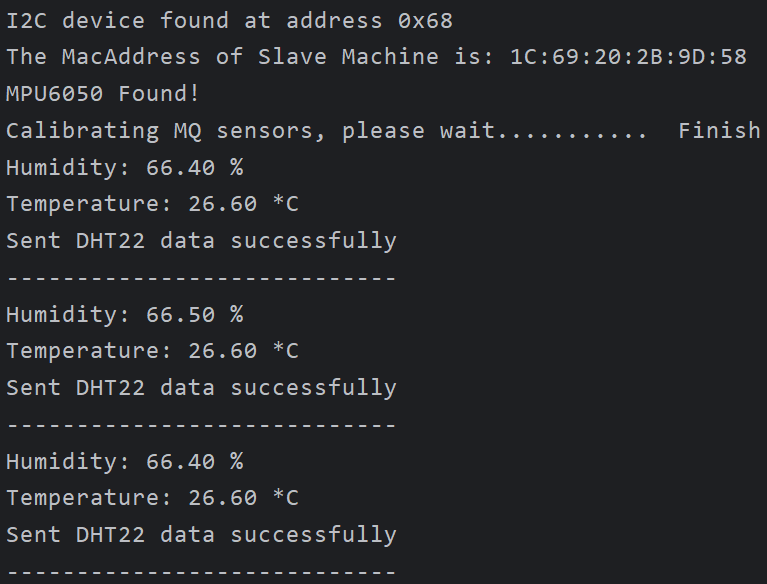
\includegraphics[width=\textwidth]{img/DHT22_active.png}
        \caption{DHT22 运行成功截图}
        \label{fig:DHT22_active}
    \end{subfigure}
    \hspace{4em}
    \begin{subfigure}[b]{0.325\textwidth}
        \centering
        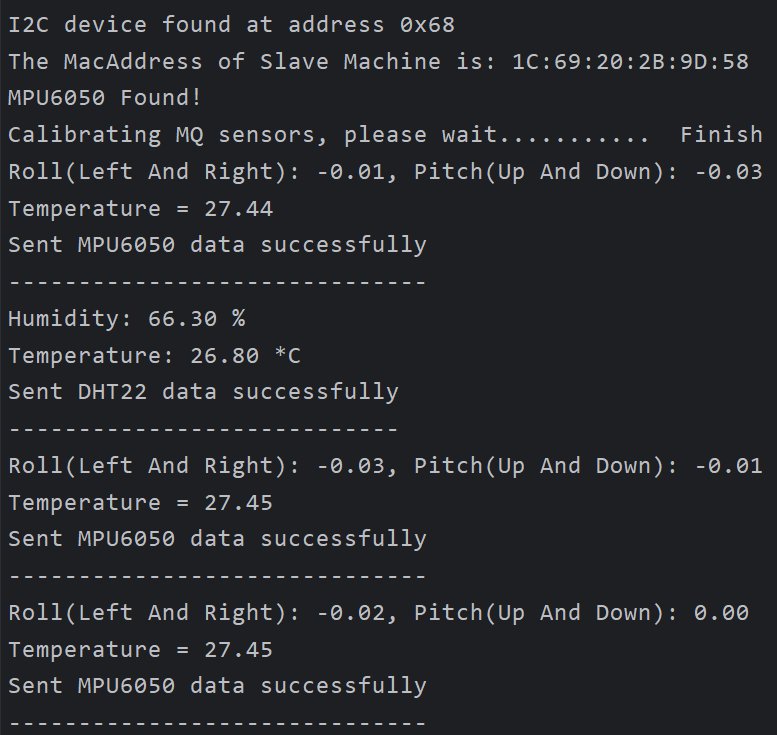
\includegraphics[width=\textwidth]{img/MPU6050_active.png}
        \caption{MPU6050 成功读取偏角}
        \label{fig:MPU6050_active}
    \end{subfigure}
    \caption{DHT22 和 MPU6050 的运行结果}
    \label{fig:combined}
\end{figure}

\subsubsection{MQ系列气体传感器}

MQUnifiedSensor库提供了各种库接口。
初次使用本库时,将ADC引脚定义为ESP32中的GPIO14,报错提示如下所示:

\begin{figure} [H]
    \centering
    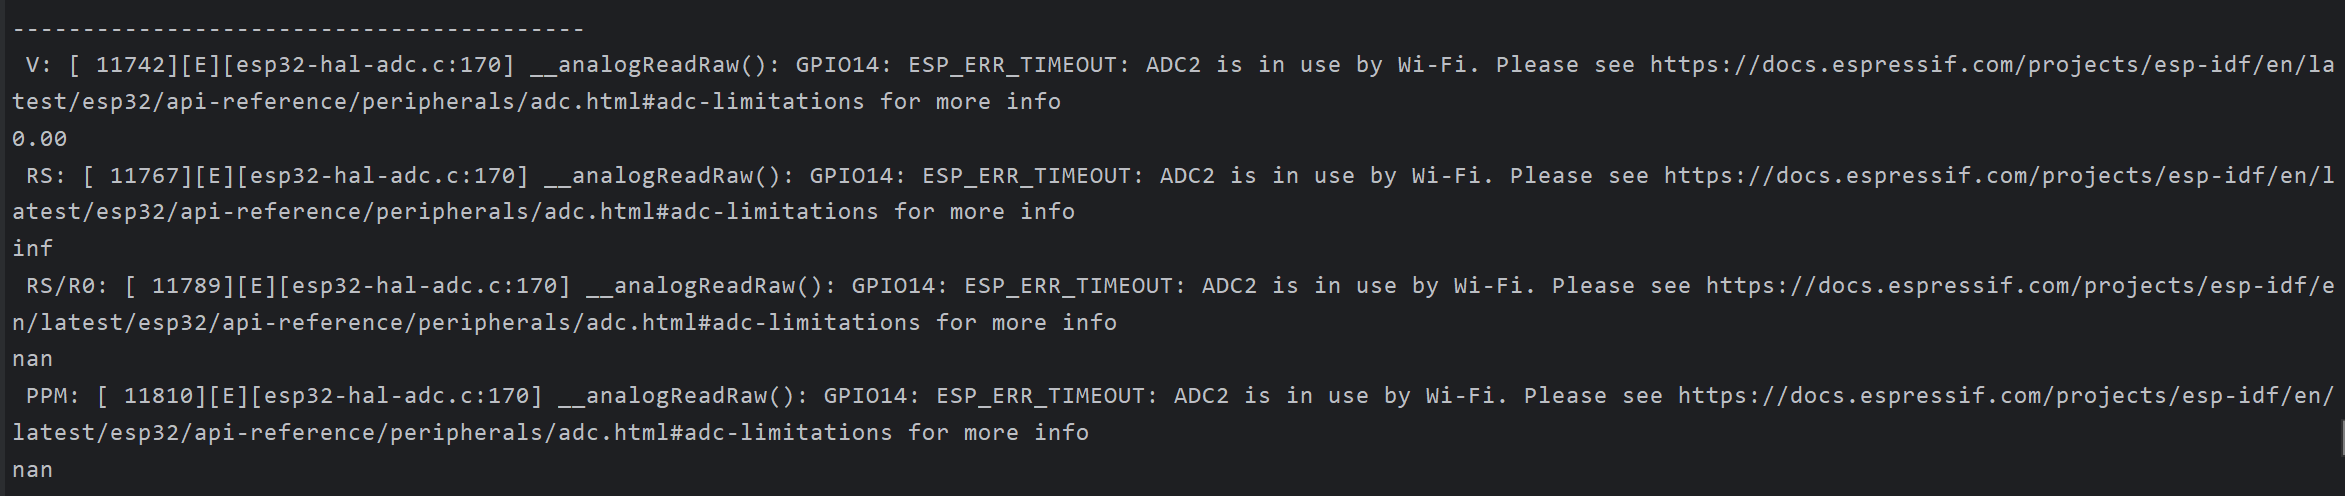
\includegraphics[width=0.8\textwidth]{img/MQ135_error.png}
    \caption{MQ135报错}
    \label{fig:MQ135_error}
\end{figure}

查阅资料后发现,Espressif(ESP32 的制造商)在设计 ESP32 时,
必须在多个功能之间做出权衡。
例如,Wi-Fi 是一个非常关键的功能,它需要稳定的时间控制和电源管理。
因此,当 Wi-Fi 活跃时,它会占用与 ADC2 共享的资源,以确保网络连接的稳定性和性能。

故将ADC模块改用为GPIO32-39即可(见\textcolor{mygreen}{附件}——ESP-Wroom-32开发板的硬件接口)

MQ-135是一种空气质量传感器,用于检测空气中的一氧化碳、氮氧化物、酒精、氨气和烟雾等有害气体。
工作原理是通过化学反应来检测目标气体的浓度,并将结果转换为电信号输出。

对于需要读取不同的气体,需要设置不同的系数(见\textcolor{mygreen}{附件})

故loop代码中应写为:

\begin{lstlisting} [language=C++, title=MQ135 不同气体的读取]
    void loopMQ135() {
        MQ135.update();
    
        // 读取 CO 浓度
        MQ135.setA(605.18);
        MQ135.setB(-3.937);
        float coPPM = MQ135.readSensor();
    
        // 读取 Alcohol 浓度
        MQ135.setA(77.255);
        MQ135.setB(-3.18);
        float alcoholPPM = MQ135.readSensor();
        // ... 重复即可
    }
\end{lstlisting}

参考自官方 MQUnifiedsensor/example/MQ-135-ALL.ino,各参数见\textcolor{mygreen}{附件}。

\begin{figure} [H]
    \centering
    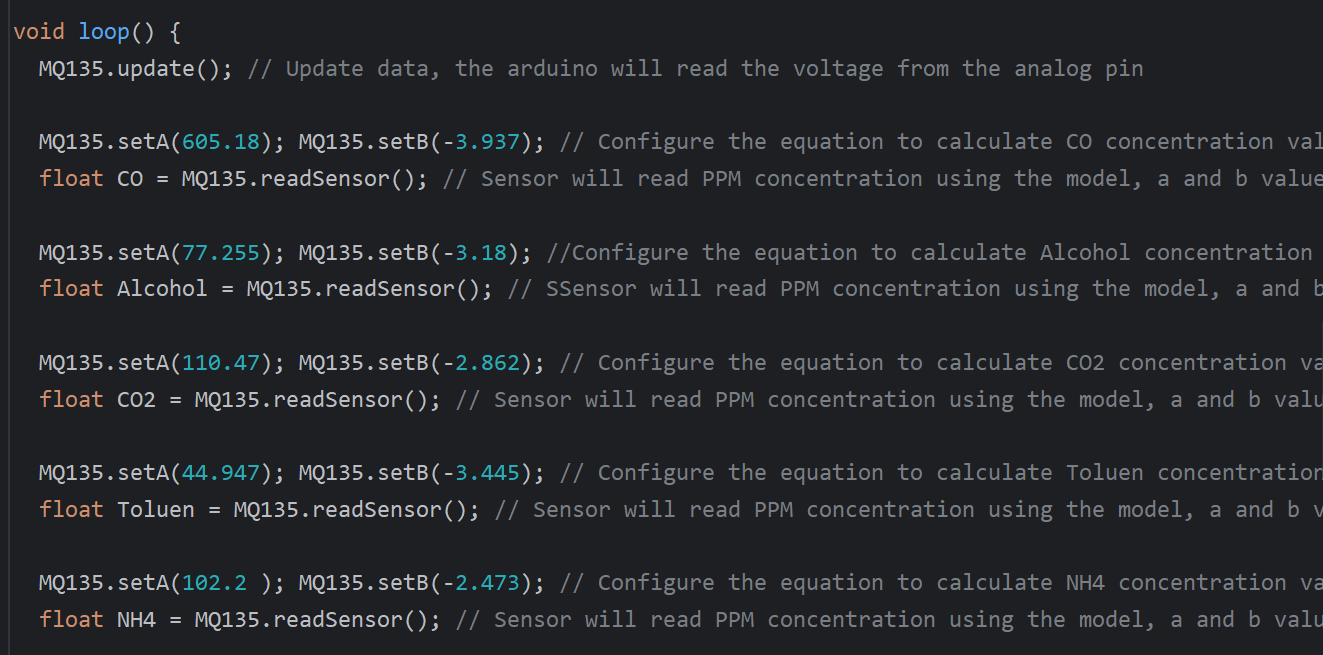
\includegraphics[width=0.5\textwidth]{img/MQ135_Para.png}
    \caption{MQ135 不同气体的系数}
    \label{fig:MQ135_coefficient}
\end{figure}

后续只需要与其他传感器相似,注册回调函数进行数据发送,即可在Master端接收到传感器带来的信息。

同理,我们可以如此操作MQ5传感器,以读取CH4、H2、LPG的PPM值(代表在空气中的浓度)。

\begin{figure} [H]
    \centering
    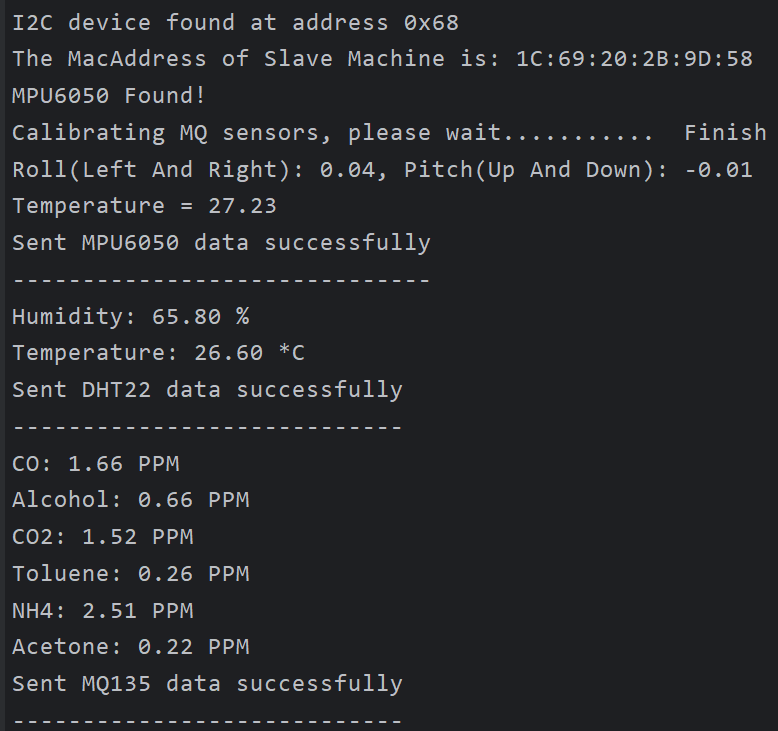
\includegraphics[width=0.4\textwidth]{img/MQ135_active.png}
    \caption{MQ135 成功读取参数}
    \label{fig:MQ135_active}
\end{figure}

\subsubsection{雨滴传感器}

雨滴传感器有两个输出口,分别是AO与DO,为了后续可以开发更多的功能,我们使用AO(Analog Output)输入。

检测是否下雨,如果下雨,则SG90舵机启动,模仿衣架收起的功能。

\subsubsection{LM393光照传感器}

光照传感器同样使用Analog Output模拟输出,为后续开发更多功能打基础。

结合雨滴传感器与光照传感器,还可以设置在夜间自动收回衣服。

\subsubsection{火焰传感器}

检测火焰的强度,在没有火焰时 Analogread() 的值为最大值,火焰越近、燃烧程度越大,得到的模拟信号值越小。